\section{State of the art}

\begin{frame}{State of the art: interval graphs}

  An \emph{interval graph} is an intersection graph of closed intervals in the real line. If the length of the intervals are the same, then it is an \emph{unit interval graph}.
  \vfill
  There exists a characterization of unit interval graphs for interval graphs.
  \begin{theorem}[Roberts]
    An interval graph is an unit interval graph if and only if it has no induced subgraph $K_{1,3}$.
  \end{theorem}
\end{frame}

\begin{frame}{State of the art: mixed unit interval graphs}

  A \emph{mixed unit interval graph} is an intersection graph of unitary intervals in the real line. The interval of mixed unit interval graphs can be open, closed, open-closed or closed-open.
  \vfill
  \pause

  \begin{figure}
  \centering
  \begin{tikzpicture}[scale=1.5]

    \draw[{(-)}] (-1,-0.5) -- (0,-0.5);
    \draw[color=black] (-0.4845,-0.8507) node {$v_4$};
    \draw[{[-}] (0,-1.5) -- (1,-1.5);
    \draw[color=black] (0.5023,-1.3568) node {$v_3$};
    \draw[{-]}] (-2,-1.5) -- (-1,-1.5);
    \draw[color=black] (-0.4899,-0.3468) node {$v_2$};
    \draw[{[-]}] (-1,-1) -- (0,-1);
    \draw[color=black] (-1.4962,-1.3536) node {$v_1$};

    \node[draw,circle,inner sep=2pt,fill,label distance=1cm] (v1) at (-4,-0.25) {};
    \draw[color=black] (-4,0) node {$v_4$};
    \node[draw,circle,inner sep=2pt,fill,label distance=1cm] (v3) at (-4,-1.25) {};
    \draw[color=black] (-4,-1.5) node {$v_2$};
    \node[draw,circle,inner sep=2pt,fill,label distance=1cm] (v2) at (-5,-1.25) {};
    \draw[color=black] (-3,-1.5) node {$v_3$};
    \node[draw,circle,inner sep=2pt,fill,label distance=1cm] (v4) at (-3,-1.25) {};
    \draw[color=black] (-5,-1.5) node {$v_1$};
    \draw  (v1) edge (v2);
    \draw  (v1) edge (v3);
    \draw  (v1) edge (v4);

  \end{tikzpicture}

  \label{fig:muigK13}
  \end{figure}
\end{frame}

\begin{frame}{State of the art: mixed unit interval graphs}
Joos characterizes mixed unit interval graphs with an exhaustive list of families of forbidden subgraphs.
\vfill

\begin{figure}
\begin{center}
  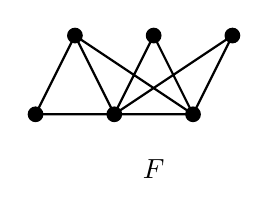
\begin{tikzpicture}[scale=1]
    \def\ver{0.1} %size of a vertex
    \def\x{1}

    \def\xa{0}
    \def\ya{0}

    %G_1
    \path[fill] (\xa+1,\ya) circle (\ver);
    \path[fill] (\xa+2,\ya) circle (\ver);
    \path[fill] (\xa+0.5,\ya+1) circle (\ver);
    \path[fill] (\xa+1.5,\ya+1) circle (\ver);
    \path[fill] (\xa+2.5,\ya+1) circle (\ver);
    \fill (\xa,\ya) circle (\ver);

    \draw[thick] (\xa+1,\ya)--(\xa+2,\ya)
    (\xa+1,\ya)--(\xa+0.5,\ya+1)--(\xa+2,\ya)
    (\xa+1,\ya)--(\xa+2.5,\ya+1)--(\xa+2,\ya)
    (\xa+1,\ya)--(\xa+1.5,\ya+1)--(\xa+2,\ya)
    (\xa+1,\ya)--(\xa,\ya)--(\xa+0.5,\ya+1);

    \node (1) at (\xa+1.5,\ya-0.7) {$F$};

\end{tikzpicture}
\end{center}
\caption{The graph $F$.}\label{fig:graphF}
\end{figure}


\end{frame}
\begin{frame}{State of the art: mixed unit interval graphs}
Joos characterizes mixed unit interval graphs with an exhaustive list of families of forbidden subgraphs.
\vfill


\begin{figure}
\begin{center}
  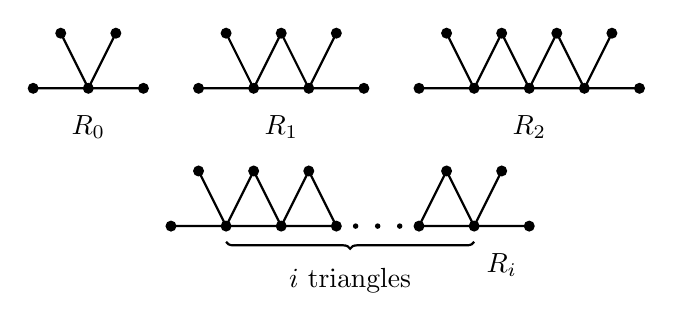
\begin{tikzpicture}[scale=0.7]
\def\ver{0.1} %size of a vertex
\def\x{1}

\def\xa{0.5}
\def\ya{0}

\def\xb{4}
\def\yb{0}

\def\xc{8}
\def\yc{0}

\def\xd{3.5}
\def\yd{-2.5}


%graph R_0
\path[fill] (\xa+0.5,\ya) circle (\ver);
\path[fill] (\xa+1,\ya+1) circle (\ver);
\path[fill] (\xa+2,\ya+1) circle (\ver);
\path[fill] (\xa+2.5,\ya) circle (\ver);
\path[fill] (\xa+1.5,\ya) circle (\ver);

\draw[thick] (\xa+0.5,\ya)--(\xa+1.5,\ya)--(\xa+1,\ya+1)
(\xa+2,\ya+1)--(\xa+1.5,\ya)--(\xa+2.5,\ya);

\node (1) at (\xa+1.5,\ya-0.7) {$R_0$};

%graph R_1
\path[fill] (\xb,\yb) circle (\ver);
\path[fill] (\xb+1,\yb) circle (\ver);
\path[fill] (\xb+2,\yb) circle (\ver);
\path[fill] (\xb+3,\yb) circle (\ver);
\path[fill] (\xb+0.5,\yb+1) circle (\ver);
\path[fill] (\xb+1.5,\yb+1) circle (\ver);
\path[fill] (\xb+2.5,\yb+1) circle (\ver);

\draw[thick] (\xb,\yb)--(\xb+1,\yb)--(\xb+2,\yb)--(\xb+3,\yb)
(\xb+0.5,\yb+1)--(\xb+1,\yb)--(\xb+1.5,\yb+1)--(\xb+2,\yb)--(\xb+2.5,\yb+1);

\node (1) at (\xb+1.5,\yb-0.7) {$R_1$};


%graph R_2
\path[fill] (\xc,\yc) circle (\ver);
\path[fill] (\xc+1,\yc) circle (\ver);
\path[fill] (\xc+2,\yc) circle (\ver);
\path[fill] (\xc+3,\yc) circle (\ver);
\path[fill] (\xc+4,\yc) circle (\ver);
\path[fill] (\xc+0.5,\yc+1) circle (\ver);
\path[fill] (\xc+1.5,\yc+1) circle (\ver);
\path[fill] (\xc+2.5,\yc+1) circle (\ver);
\path[fill] (\xc+3.5,\yc+1) circle (\ver);

\draw[thick] (\xc,\yc)--(\xc+1,\yc)--(\xc+2,\yc)--(\xc+3,\yc)--(\xc+4,\yc)
(\xc+0.5,\yc+1)--(\xc+1,\yc)--(\xc+1.5,\yc+1)--(\xc+2,\yc)--(\xc+2.5,\yc+1)--(\xc+3,\yc)--(\xc+3.5,\yc+1);

\node (1) at (\xc+2,\yc-0.7) {$R_2$};

%graph R_i
\path[fill] (\xd,\yd) circle (\ver);
\path[fill] (\xd+1,\yd) circle (\ver);
\path[fill] (\xd+2,\yd) circle (\ver);
\path[fill] (\xd+3,\yd) circle (\ver);
\path[fill] (\xd+4.5,\yd) circle (\ver);
\path[fill] (\xd+5.5,\yd) circle (\ver);
\path[fill] (\xd+6.5,\yd) circle (\ver);
\path[fill] (\xd+0.5,\yd+1) circle (\ver);
\path[fill] (\xd+1.5,\yd+1) circle (\ver);
\path[fill] (\xd+2.5,\yd+1) circle (\ver);
\path[fill] (\xd+5,\yd+1) circle (\ver);
\path[fill] (\xd+6,\yd+1) circle (\ver);

\fill (\xd+3.35,\yd) circle (\ver/2);
\fill (\xd+3.75,\yd) circle (\ver/2);
\fill (\xd+4.15,\yd) circle (\ver/2);

\draw[thick] (\xd,\yd)--(\xd+3,\yd)
(\xd+4.5,\yd)--(\xd+6.5,\yd)
(\xd+0.5,\yd+1)--(\xd+1,\yd)--(\xd+1.5,\yd+1)--(\xd+2,\yd)--(\xd+2.5,\yd+1)--(\xd+3,\yd)
(\xd+4.5,\yd)--(\xd+5,\yd+1)--(\xd+5.5,\yd)--(\xd+6,\yd+1);

\draw[thick,decoration={brace,mirror,raise=0.2cm},decorate] (\xd+1,\yd) -- (\xd+5.5,\yd)
node [pos=0.5,anchor=north,yshift=-0.4cm] {$i$ triangles};

\node (1) at (\xd+6,\yd-0.7) {$R_i$};

\end{tikzpicture}
\end{center}
\caption{The family $\mathcal{R}$.}\label{fig:graphsR}
\end{figure}



\end{frame}
\begin{frame}{State of the art: mixed unit interval graphs}
Joos characterizes mixed unit interval graphs with an exhaustive list of families of forbidden subgraphs.
\vfill

\begin{figure}[t]
\begin{center}
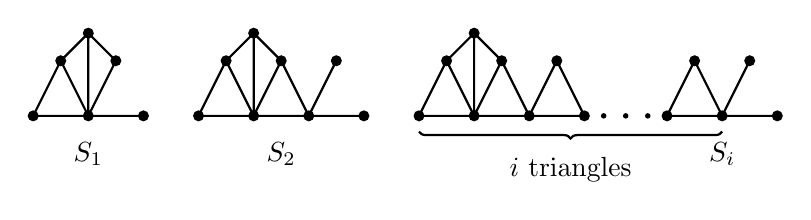
\begin{tikzpicture}[scale=0.7]
\def\ver{0.1} %size of a vertex
\def\x{1}

\def\xa{0}
\def\ya{0}

\def\xb{0}
\def\yb{0}

\def\xc{4}
\def\yc{0}

\def\xd{9}
\def\yd{0}


%graph S_1
\path[fill] (\xb+1,\yb) circle (\ver);
\path[fill] (\xb+2,\yb) circle (\ver);
\path[fill] (\xb+3,\yb) circle (\ver);
\path[fill] (\xb+2,\yb+1.5) circle (\ver);
\path[fill] (\xb+1.5,\yb+1) circle (\ver);
\path[fill] (\xb+2.5,\yb+1) circle (\ver);

\draw[thick] (\xb+1,\yb)--(\xb+2,\yb)--(\xb+3,\yb)
(\xb+1,\yb)--(\xb+1.5,\yb+1)--(\xb+2,\yb)--(\xb+2.5,\yb+1)
--(\xb+2,\yb+1.5)--(\xb+2,\yb)
(\xb+1.5,\yb+1)--(\xb+2,\yb+1.5);

\node (1) at (\xb+2,\yb-0.7) {$S_1$};



%graph S_2
\path[fill] (\xc,\yc) circle (\ver);
\path[fill] (\xc+1,\yc) circle (\ver);
\path[fill] (\xc+2,\yc) circle (\ver);
\path[fill] (\xc+3,\yc) circle (\ver);
\path[fill] (\xc+0.5,\yc+1) circle (\ver);
\path[fill] (\xc+1.5,\yc+1) circle (\ver);
\path[fill] (\xc+2.5,\yc+1) circle (\ver);
\path[fill] (\xc+1,\yc+1.5) circle (\ver);


\draw[thick] (\xc,\yc)--(\xc+1,\yc)--(\xc+2,\yc)--(\xc+3,\yc)
(\xc+0.5,\yc+1)--(\xc+1,\yc)--(\xc+1.5,\yc+1)--(\xc+2,\yc)--(\xc+2.5,\yc+1)
(\xc,\yc)--(\xc+0.5,\yc+1)--(\xc+1,\yc+1.5)--(\xc+1.5,\yc+1)
(\xc+1,\yc)--(\xc+1,\yc+1.5);

\node (1) at (\xc+1.5,\yc-0.7) {$S_2$};

%graph S_3
\path[fill] (\xd-1,\yd) circle (\ver);
\path[fill] (\xd-0.5,\yd+1) circle (\ver);
\path[fill] (\xd,\yd) circle (\ver);
\path[fill] (\xd+1,\yd) circle (\ver);
\path[fill] (\xd+2,\yd) circle (\ver);
\path[fill] (\xd+3.5,\yd) circle (\ver);
\path[fill] (\xd+4.5,\yd) circle (\ver);
\path[fill] (\xd+5.5,\yd) circle (\ver);
\path[fill] (\xd+0.5,\yd+1) circle (\ver);
\path[fill] (\xd+1.5,\yd+1) circle (\ver);
\path[fill] (\xd+4,\yd+1) circle (\ver);
\path[fill] (\xd+5,\yd+1) circle (\ver);
\path[fill] (\xd,\yd+1.5) circle (\ver);

\fill (\xd+2.35,\yd) circle (\ver/2);
\fill (\xd+2.75,\yd) circle (\ver/2);
\fill (\xd+3.15,\yd) circle (\ver/2);

\draw[thick] (\xd-1,\yd)--(\xd+2,\yd)
(\xd+3.5,\yd)--(\xd+5.5,\yd)
(\xd-1,\yd)--(\xd-0.5,\yd+1)--(\xd,\yd)--(\xd+0.5,\yd+1)--(\xd+1,\yd)--(\xd+1.5,\yd+1)--(\xd+2,\yd)
(\xd+3.5,\yd)--(\xd+4,\yd+1)--(\xd+4.5,\yd)--(\xd+5,\yd+1)
(\xd-0.5,\yd+1)--(\xd,\yd+1.5)--(\xd+0.5,\yd+1)
(\xd,\yd)--(\xd,\yd+1.5);

\draw[thick,decoration={brace,mirror,raise=0.2cm},decorate] (\xd-1,\yd) -- (\xd+4.5,\yd)
node [pos=0.5,anchor=north,yshift=-0.4cm] {$i$ triangles};

\node (1) at (\xd+4.5,\yd-0.7) {$S_i$};



\end{tikzpicture}
\end{center}
\caption{The family $\mathcal{S}$.}\label{fig:graphsS}
\end{figure}



\end{frame}
\begin{frame}{State of the art: mixed unit interval graphs}
Joos characterizes mixed unit interval graphs with an exhaustive list of families of forbidden subgraphs.
\vfill

\begin{figure}
\begin{center}
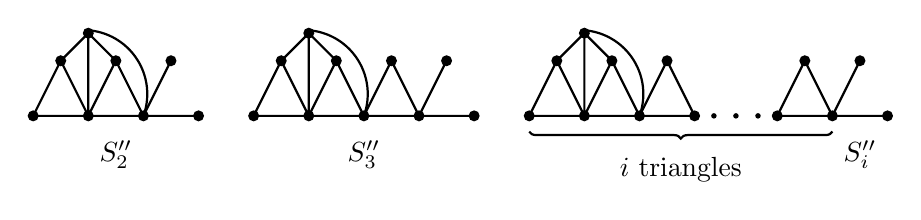
\begin{tikzpicture}[scale=0.7]
\def\ver{0.1} %size of a vertex
\def\x{1}

\def\xa{10}
\def\ya{0}

\def\xb{0}
\def\yb{0}

\def\xc{0}
\def\yc{0}

\def\xd{5}
\def\yd{0}

%graph S^2_2
\path[fill] (\xc,\yc) circle (\ver);
\path[fill] (\xc+1,\yc) circle (\ver);
\path[fill] (\xc+2,\yc) circle (\ver);
\path[fill] (\xc+3,\yc) circle (\ver);
\path[fill] (\xc+0.5,\yc+1) circle (\ver);
\path[fill] (\xc+1.5,\yc+1) circle (\ver);
\path[fill] (\xc+2.5,\yc+1) circle (\ver);
\path[fill] (\xc+1,\yc+1.5) circle (\ver);


\draw[thick] (\xc,\yc)--(\xc+1,\yc)--(\xc+2,\yc)--(\xc+3,\yc)
(\xc+0.5,\yc+1)--(\xc+1,\yc)--(\xc+1.5,\yc+1)--(\xc+2,\yc)--(\xc+2.5,\yc+1)
(\xc,\yc)--(\xc+0.5,\yc+1)--(\xc+1,\yc+1.5)--(\xc+1.5,\yc+1)
(\xc+1,\yc)--(\xc+1,\yc+1.5);

\draw[thick] (\xc+2,\yc) arc(-20:85:1.16);

\node (1) at (\xc+1.5,\yc-0.7) {$S_2''$};

%graph S^2_3
\path[fill] (\xd-1,\yd) circle (\ver);
\path[fill] (\xd-0.5,\yd+1) circle (\ver);
\path[fill] (\xd,\yd) circle (\ver);
\path[fill] (\xd+1,\yd) circle (\ver);
\path[fill] (\xd+2,\yd) circle (\ver);
\path[fill] (\xd+3,\yd) circle (\ver);
\path[fill] (\xd+0.5,\yd+1) circle (\ver);
\path[fill] (\xd+1.5,\yd+1) circle (\ver);
\path[fill] (\xd+2.5,\yd+1) circle (\ver);
\path[fill] (\xd,\yd+1.5) circle (\ver);


\draw[thick] (\xd-1,\yd)--(\xd+3,\yd)
(\xd-1,\yd)--(\xd-0.5,\yd+1)--(\xd,\yd)--(\xd+0.5,\yd+1)--(\xd+1,\yd)--(\xd+1.5,\yd+1)--(\xd+2,\yd)--(\xd+2.5,\yd+1)
(\xd-0.5,\yd+1)--(\xd,\yd+1.5)--(\xd+0.5,\yd+1)
(\xd,\yd)--(\xd,\yd+1.5);

\draw[thick] (\xd+1,\yd) arc(-20:85:1.16);

\node (1) at (\xd+1,\yd-0.7) {$S_3''$};

%graph S_i''
\path[fill] (\xa-1,\ya) circle (\ver);
\path[fill] (\xa,\ya) circle (\ver);
\path[fill] (\xa+1,\ya) circle (\ver);
\path[fill] (\xa+2,\ya) circle (\ver);
\path[fill] (\xa+3.5,\ya) circle (\ver);
\path[fill] (\xa+4.5,\ya) circle (\ver);
\path[fill] (\xa+5.5,\ya) circle (\ver);
\path[fill] (\xa-0.5,\ya+1) circle (\ver);
\path[fill] (\xa+0.5,\ya+1) circle (\ver);
\path[fill] (\xa+1.5,\ya+1) circle (\ver);
\path[fill] (\xa+4,\ya+1) circle (\ver);
\path[fill] (\xa+5,\ya+1) circle (\ver);
\path[fill] (\xa,\ya+1.5) circle (\ver);


\draw[thick] (\xa-1,\ya)--(\xa+2,\ya)
(\xa+3.5,\ya)--(\xa+5.5,\ya)
(\xa-1,\ya)--(\xa-0.5,\ya+1)--(\xa,\ya)--(\xa+0.5,\ya+1)--(\xa+1,\ya)--(\xa+1.5,\ya+1)--(\xa+2,\ya)
(\xa+3.5,\ya)--(\xa+4,\ya+1)--(\xa+4.5,\ya)--(\xa+5,\ya+1)
(\xa-0.5,\ya+1)--(\xa,\ya+1.5)--(\xa+0.5,\ya+1)
(\xa,\ya)--(\xa,\ya+1.5);

\draw[thick] (\xa+1,\ya) arc(-20:85:1.16);

\node (1) at (\xa+5,\ya-0.7) {$S_i''$};

\fill (\xa+2.35,\ya) circle (\ver/2);
\fill (\xa+2.75,\ya) circle (\ver/2);
\fill (\xa+3.15,\ya) circle (\ver/2);

\draw[thick,decoration={brace,mirror,raise=0.2cm},decorate] (\xa-1,\ya) -- (\xa+4.5,\ya)
node [pos=0.5,anchor=north,yshift=-0.4cm] {$i$ triangles};

\end{tikzpicture}
\end{center}
\caption{The family $\mathcal{S}''$.}\label{fig:graphsSS}
\end{figure}


\end{frame}
\begin{frame}{State of the art: mixed unit interval graphs}
Joos characterizes mixed unit interval graphs with an exhaustive list of families of forbidden subgraphs.
\vfill

\begin{figure}
\begin{center}
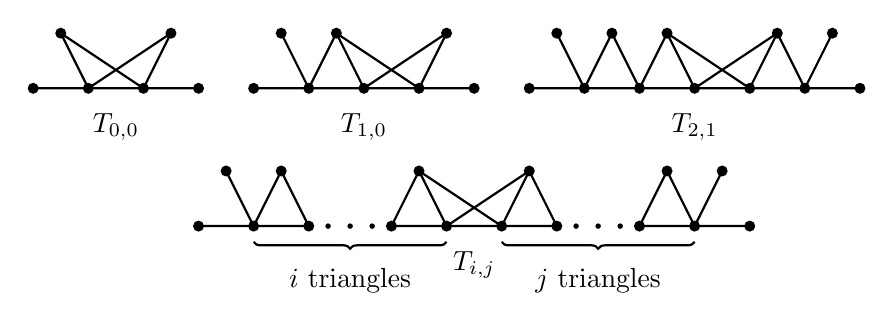
\begin{tikzpicture}[scale=0.7]
\def\ver{0.1} %size of a vertex
\def\x{1}

\def\xa{0}
\def\ya{0}

\def\xb{4}
\def\yb{0}

\def\xc{9}
\def\yc{0}

\def\xd{3}
\def\yd{-2.5}

%graph T_{0,0}
\path[fill] (\xa,\ya) circle (\ver);
\path[fill] (\xa+1,\ya) circle (\ver);
\path[fill] (\xa+2,\ya) circle (\ver);
\path[fill] (\xa+3,\ya) circle (\ver);
\path[fill] (\xa+0.5,\ya+1) circle (\ver);
\path[fill] (\xa+2.5,\ya+1) circle (\ver);

\draw[thick] (\xa,\ya)--(\xa+3,\ya)
(\xa+1,\ya)--(\xa+0.5,\ya+1)--(\xa+2,\ya)
(\xa+1,\ya)--(\xa+2.5,\ya+1)--(\xa+2,\ya);

\node (1) at (\xa+1.5,\ya-0.7) {$T_{0,0}$};

%graph T_{1,0}
\path[fill] (\xb,\yb) circle (\ver);
\path[fill] (\xb+1,\yb) circle (\ver);
\path[fill] (\xb+2,\yb) circle (\ver);
\path[fill] (\xb+3,\yb) circle (\ver);
\path[fill] (\xb+4,\yb) circle (\ver);
\path[fill] (\xb+0.5,\yb+1) circle (\ver);
\path[fill] (\xb+1.5,\yb+1) circle (\ver);
\path[fill] (\xb+3.5,\yb+1) circle (\ver);

\draw[thick] (\xb,\yb)--(\xb+4,\yb)
(\xb+0.5,\yb+1)--(\xb+1,\yb)--(\xb+1.5,\yb+1)--(\xb+2,\yb)--(\xb+3.5,\yb+1)
--(\xb+3,\yb)--(\xb+1.5,\yb+1);

\node (1) at (\xb+2,\yb-0.7) {$T_{1,0}$};

%graph T_{2,1}
\path[fill] (\xc,\yc) circle (\ver);
\path[fill] (\xc+1,\yc) circle (\ver);
\path[fill] (\xc+2,\yc) circle (\ver);
\path[fill] (\xc+3,\yc) circle (\ver);
\path[fill] (\xc+4,\yc) circle (\ver);
\path[fill] (\xc+5,\yc) circle (\ver);
\path[fill] (\xc+6,\yc) circle (\ver);
\path[fill] (\xc+0.5,\yc+1) circle (\ver);
\path[fill] (\xc+1.5,\yc+1) circle (\ver);
\path[fill] (\xc+2.5,\yc+1) circle (\ver);
\path[fill] (\xc+4.5,\yc+1) circle (\ver);
\path[fill] (\xc+5.5,\yc+1) circle (\ver);

\draw[thick] (\xc,\yc)--(\xc+6,\yc)
(\xc+0.5,\yc+1)--(\xc+1,\yc)--(\xc+1.5,\yc+1)--(\xc+2,\yc)--(\xc+2.5,\yc+1)--(\xc+3,\yc)--(\xc+4.5,\yc+1)
(\xc+5.5,\yc+1)--(\xc+5,\yc)--(\xc+4.5,\yc+1)--(\xc+4,\yc)--(\xc+2.5,\yc+1);

\node (1) at (\xc+3,\yc-0.7) {$T_{2,1}$};

%graph T_{i,j}
\path[fill] (\xd,\yd) circle (\ver);
\path[fill] (\xd+1,\yd) circle (\ver);
\path[fill] (\xd+2,\yd) circle (\ver);
\path[fill] (\xd+3.5,\yd) circle (\ver);
\path[fill] (\xd+4.5,\yd) circle (\ver);
\path[fill] (\xd+5.5,\yd) circle (\ver);
\path[fill] (\xd+6.5,\yd) circle (\ver);
\path[fill] (\xd+8,\yd) circle (\ver);
\path[fill] (\xd+9,\yd) circle (\ver);
\path[fill] (\xd+10,\yd) circle (\ver);
\path[fill] (\xd+0.5,\yd+1) circle (\ver);
\path[fill] (\xd+1.5,\yd+1) circle (\ver);
\path[fill] (\xd+4,\yd+1) circle (\ver);
\path[fill] (\xd+6,\yd+1) circle (\ver);
\path[fill] (\xd+8.5,\yd+1) circle (\ver);
\path[fill] (\xd+9.5,\yd+1) circle (\ver);

\draw[thick] (\xd,\yd)--(\xd+2,\yd)
(\xd+3.5,\yd)--(\xd+6.5,\yd)
(\xd+8,\yd)--(\xd+10,\yd)
(\xd+0.5,\yd+1)--(\xd+1,\yd)--(\xd+1.5,\yd+1)--(\xd+2,\yd)
(\xd+8,\yd)--(\xd+8.5,\yd+1)--(\xd+9,\yd)--(\xd+9.5,\yd+1)
(\xd+3.5,\yd)--(\xd+4,\yd+1)--(\xd+4.5,\yd)
(\xd+5.5,\yd)--(\xd+6,\yd+1)--(\xd+6.5,\yd)
(\xd+4,\yd+1)--(\xd+5.5,\yd)
(\xd+6,\yd+1)--(\xd+4.5,\yd);

\fill (\xd+2.35,\yd) circle (\ver/2);
\fill (\xd+2.75,\yd) circle (\ver/2);
\fill (\xd+3.15,\yd) circle (\ver/2);

\fill (\xd+6.85,\yd) circle (\ver/2);
\fill (\xd+7.25,\yd) circle (\ver/2);
\fill (\xd+7.65,\yd) circle (\ver/2);

\draw[thick,decoration={brace,mirror,raise=0.2cm},decorate] (\xd+1,\yd) -- (\xd+4.5,\yd)
node [pos=0.5,anchor=north,yshift=-0.4cm] {$i$ triangles};

\draw[thick,decoration={brace,mirror,raise=0.2cm},decorate] (\xd+5.5,\yd) -- (\xd+9,\yd)
node [pos=0.5,anchor=north,yshift=-0.4cm] {$j$ triangles};


\node (1) at (\xd+5,\yd-0.7) {$T_{i,j}$};

\end{tikzpicture}
\end{center}
\caption{The family $\mathcal{T}$.}\label{fig:graphsT}
\end{figure}

\end{frame}

\begin{frame}{State of the art: unfettered unit interval graphs}
  An \emph{unfettered unit interval graph} is an intersection graph of unitary intervals in the real line. However, if two intervals \emph{kiss}, we can choose whether they are adjacent or not.
  \vfill
  \pause
  \begin{columns}
    \begin{column}{0.5\textwidth}
  \begin{figure}
  \centering
  \begin{tikzpicture}[scale=1.5]

    \draw[{>-<}] (-1,-0.5) -- (0,-0.5);
    \draw[color=black] (-0.4845,-0.8507) node {$v_4$};
    \draw[{>-}] (0,-1.5) -- (1,-1.5);
    \draw[color=black] (0.5023,-1.3568) node {$v_3$};
    \draw[{-<}] (-2,-1.5) -- (-1,-1.5);
    \draw[color=black] (-0.4899,-0.3468) node {$v_2$};
    \draw[{>-<}] (-1,-1) -- (0,-1);
    \draw[color=black] (-1.4962,-1.3536) node {$v_1$};
    \draw[color=red, dashed] (-1,-2) -- (-1,0);
    \draw[color=red, dashed] (0,-2) -- (0,0);

  \end{tikzpicture}
  \label{fig:muigK13}
  \end{figure}
\end{column}
\pause
\begin{column}{0.5\textwidth}
\begin{columns}
  \begin{column}{0.5\textwidth}
  \begin{figure}
  \centering
  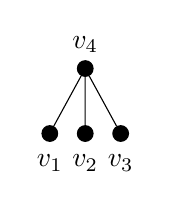
\begin{tikzpicture}[scale=1.5]

  \node[draw,circle,inner sep=2pt,fill,label distance=1cm] (v1) at (-4,-0.7) {};
  \draw[color=black] (-4,-0.5) node {$v_4$};
  \node[draw,circle,inner sep=2pt,fill,label distance=1cm] (v3) at (-4,-1.25) {};
  \draw[color=black] (-4,-1.5) node {$v_2$};
  \node[draw,circle,inner sep=2pt,fill,label distance=1cm] (v2) at (-4.3,-1.25) {};
  \draw[color=black] (-3.7,-1.5) node {$v_3$};
  \node[draw,circle,inner sep=2pt,fill,label distance=1cm] (v4) at (-3.7,-1.25) {};
  \draw[color=black] (-4.3,-1.5) node {$v_1$};
  \draw  (v1) edge (v2);
  \draw  (v1) edge (v3);
  \draw  (v1) edge (v4);

\end{tikzpicture}
\label{fig:muigK13}
\end{figure}
\vfill
\pause
\begin{figure}
\centering
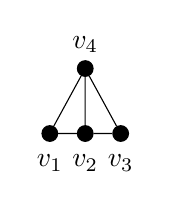
\begin{tikzpicture}[scale=1.5]

\node[draw,circle,inner sep=2pt,fill,label distance=1cm] (v1) at (-4,-0.7) {};
\draw[color=black] (-4,-0.5) node {$v_4$};
\node[draw,circle,inner sep=2pt,fill,label distance=1cm] (v3) at (-4,-1.25) {};
\draw[color=black] (-4,-1.5) node {$v_2$};
\node[draw,circle,inner sep=2pt,fill,label distance=1cm] (v2) at (-4.3,-1.25) {};
\draw[color=black] (-3.7,-1.5) node {$v_3$};
\node[draw,circle,inner sep=2pt,fill,label distance=1cm] (v4) at (-3.7,-1.25) {};
\draw[color=black] (-4.3,-1.5) node {$v_1$};
\draw  (v1) edge (v2);
\draw  (v1) edge (v3);
\draw  (v2) edge (v3);
\draw  (v3) edge (v4);
\draw  (v1) edge (v4);

\end{tikzpicture}
\label{fig:muigK13}
\end{figure}
\end{column}
\pause
\begin{column}{0.5\textwidth}

\begin{figure}
\centering
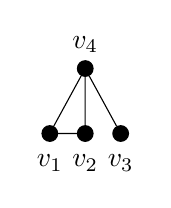
\begin{tikzpicture}[scale=1.5]

\node[draw,circle,inner sep=2pt,fill,label distance=1cm] (v1) at (-4,-0.7) {};
\draw[color=black] (-4,-0.5) node {$v_4$};
\node[draw,circle,inner sep=2pt,fill,label distance=1cm] (v3) at (-4,-1.25) {};
\draw[color=black] (-4,-1.5) node {$v_2$};
\node[draw,circle,inner sep=2pt,fill,label distance=1cm] (v2) at (-4.3,-1.25) {};
\draw[color=black] (-3.7,-1.5) node {$v_3$};
\node[draw,circle,inner sep=2pt,fill,label distance=1cm] (v4) at (-3.7,-1.25) {};
\draw[color=black] (-4.3,-1.5) node {$v_1$};
\draw  (v1) edge (v2);
\draw  (v1) edge (v3);
\draw  (v2) edge (v3);
\draw  (v1) edge (v4);

\end{tikzpicture}
\label{fig:muigK13}
\end{figure}

\vfill
\pause

\begin{figure}
\centering
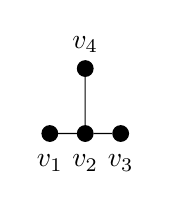
\begin{tikzpicture}[scale=1.5]

\node[draw,circle,inner sep=2pt,fill,label distance=1cm] (v1) at (-4,-0.7) {};
\draw[color=black] (-4,-0.5) node {$v_4$};
\node[draw,circle,inner sep=2pt,fill,label distance=1cm] (v3) at (-4,-1.25) {};
\draw[color=black] (-4,-1.5) node {$v_2$};
\node[draw,circle,inner sep=2pt,fill,label distance=1cm] (v2) at (-4.3,-1.25) {};
\draw[color=black] (-3.7,-1.5) node {$v_3$};
\node[draw,circle,inner sep=2pt,fill,label distance=1cm] (v4) at (-3.7,-1.25) {};
\draw[color=black] (-4.3,-1.5) node {$v_1$};
\draw  (v1) edge (v3);
\draw  (v2) edge (v3);
\draw  (v3) edge (v4);

\end{tikzpicture}
\label{fig:muigK13}
\end{figure}
\end{column}
\end{columns}

\end{column}
\end{columns}

\end{frame}

\begin{frame}{State of the art: unfettered unit interval graphs}
  This class has been completely characterized by its structure.

  \begin{theorem}[Hayashi]
      A graph $G$ is a unfettered unit interval graph if and only if it has a level structure where every level is a clique.
  \end{theorem}
  \vfill
  \begin{definition}
    A \emph{level structure} of a graph $G = (V,E)$ is a partition $L = \{L_i : i \in \{1,\dots, t\}\}$ of $V$ such that

    $$v \in L_k \Rightarrow N(v) \subseteq L_{k-1} \cup L_{k} \cup L_{k+1}$$

    where $L_0 = L_{t+1} = \varnothing$.
  \end{definition}
\end{frame}

\begin{frame}{State of the art: unit disk graphs}
  A \emph{disk graph} is an intersection graph of closed intervals in the real line. If the length of the intervals are the same, then it is an \emph{unit disk graph}.
  \vfill
  \begin{figure}
  \centering

  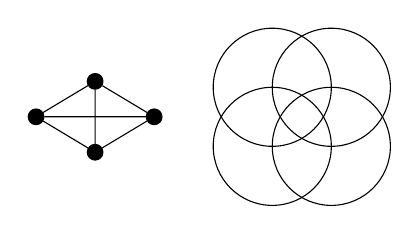
\begin{tikzpicture}[scale=1.5]

    \draw (-0.5,2.5) circle [radius=0.5];
    \draw (0,2.5) circle [radius=0.5];
    \draw (-0.5,2) circle [radius=0.5];
    \draw (0,2) circle [radius=0.5];


    \node[draw,circle,inner sep=2pt,fill,label distance=1cm] (v1) at (-2.5,2.25) {};

    \node[draw,circle,inner sep=2pt,fill,label distance=1cm] (v2) at (-2,1.95) {};
    \node[draw,circle,inner sep=2pt,fill,label distance=1cm] (v3) at (-2,2.55) {};
    \node[draw,circle,inner sep=2pt,fill,label distance=1cm] (v4) at (-1.5,2.25) {};

    \draw  (v3) edge (v2);
    \draw  (v4) edge (v1);
    \draw  (v3) edge (v1);
    \draw  (v4) edge (v2);
    \draw  (v3) edge (v4);
    \draw  (v1) edge (v2);

  \end{tikzpicture}
  \label{fig:udg}
  \end{figure}
\end{frame}

\begin{frame}{State of the art: $c$-strip graphs}
  A \emph{$c$-strip graph} - or SG($c$) is a unit disk graph such that the centers of each disk belong to $\{(x,y) : -\infty < x < \infty, 0 \leq y \leq c\}$
  \vfill
  \pause
  \begin{remark}
    $\text{SG}(0) = \text{UIG}$.
  \end{remark}
  \begin{remark}
    $\text{SG}(\infty) = \text{UDG}$.
  \end{remark}
  \begin{remark}
    $\text{SG}(k) \subseteq \text{SG}(l)$ with $k < l$.
  \end{remark}

\end{frame}

\begin{frame}{State of the art: thin strip graphs}
  The class of \emph{thin strip graphs} is the intersection of every $c$-strip graph with $c > 0$. Thus, a $\varepsilon$-strip graph with $\varepsilon$ arbitrarily small.
  \vfill
  \begin{figure}
  \centering
  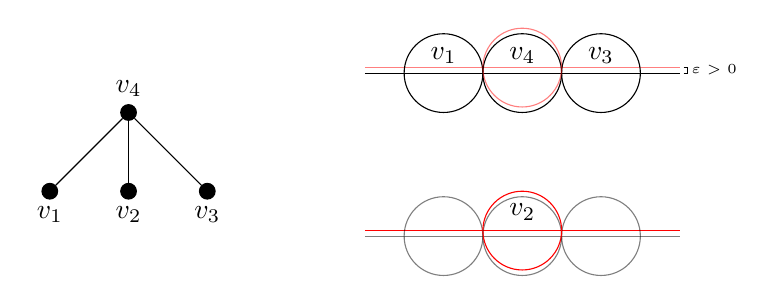
\begin{tikzpicture}[scale=1]

  \draw (-2,0) -- (2,0);
  \draw[red ,opacity = 0.5] (-2,0.07) -- (2,0.07);
  \draw  (-1,0) circle [radius=0.5];
  \draw[color=black] (-1,0.2265) node {$v_1$};
  \draw  (0,0) circle [radius=0.5];
  \draw[color=black] (0,0.2265) node {$v_4$};
  \draw  (1,0) circle [radius=0.5];
  \draw[color=black] (1,0.2265) node {$v_3$};

  \draw[red, opacity = 0.5] (0,0.07) circle [radius=0.5];
  \draw[color=black] (2.4386,0.0367) node {\tiny $\varepsilon > 0$};

  % lines to describe distance (epsilon)
  \draw[very thin] (2.1,0.07) -- (2.1,0);
  \draw[very thin] (2.05,0.07) -- (2.1,0.07);
  \draw[very thin] (2.05,0) -- (2.1,0);

  \draw[opacity = 0.5] (-2,-2.07) -- (2,-2.07);
  \draw[red] (-2,-2) -- (2,-2);
  \draw[opacity = 0.5]  (0,-2.07) circle [radius=0.5];
  \draw[opacity = 0.5]  (1,-2.07) circle [radius=0.5];
  \draw[opacity = 0.5]  (-1,-2.07) circle [radius=0.5];
  \draw[red] (0,-2) circle [radius=0.5];
  \draw[color=black] (0,-1.765) node {$v_2$};

  \node[draw,circle,inner sep=2pt,fill,label distance=1cm] (v1) at (-5,-0.5) {};
  \draw[color=black] (-5,-0.2) node {$v_4$};
  \node[draw,circle,inner sep=2pt,fill,label distance=1cm] (v3) at (-5,-1.5) {};
  \draw[color=black] (-5,-1.8) node {$v_2$};
  \node[draw,circle,inner sep=2pt,fill,label distance=1cm] (v2) at (-6,-1.5) {};
  \draw[color=black] (-4,-1.8) node {$v_3$};
  \node[draw,circle,inner sep=2pt,fill,label distance=1cm] (v4) at (-4,-1.5) {};
  \draw[color=black] (-6,-1.8) node {$v_1$};
  \draw  (v1) edge (v2);
  \draw  (v1) edge (v3);
  \draw  (v1) edge (v4);
  \end{tikzpicture}
  \label{fig:thinK13}
  \end{figure}
\end{frame}

\begin{frame}{State of the art: thin strip graphs}
  Hayashi \textit{et al.} introduced the class of \textit{thin strip graphs}. They also found these important results about $c$-strip graphs and thin strip graphs.
  \vfill
  \begin{theorem}
    There is no constant $t$ such that $\text{SG}(t) = \text{TSG}$.
  \end{theorem}
  \begin{theorem}
    There is no constant $t$ such that $\text{SG}(t) = \text{UDG}$.
  \end{theorem}
  \pause
  In order to prove these theorems, they proved that a forbidden subgraph of MUIG is also forbidden in TSG.
\end{frame}

\begin{frame}{State of the art: thin strip graphs}
  Hayashi \textit{et al.} introduced the class of \textit{thin strip graphs}. They also found these important results about $c$-strip graphs and thin strip graphs.
  \vfill
  \begin{theorem}
    Mixed unit interval graphs is a subclass of thin strip graphs.
  \end{theorem}
  \begin{theorem}
    Thin strip graphs is a subclass of unfettered unit interval graphs.
  \end{theorem}
\end{frame}

\begin{frame}{State of the art: thin strip graphs}
  \begin{figure}
  \begin{center}
  \begin{tikzpicture}[scale=1]
    \node (1) [draw, rounded rectangle] {unfettered unit interval graphs};
    \node (2) [below=of 1, draw, rounded rectangle] {thin strip graphs};
    \node (3) [below=of 2, draw, rounded rectangle] {mixed unit interval graphs};
    \node (4) [below=of 3, draw, rounded rectangle] {unit interval graphs};
    \node (5) [left=of 1, draw, rounded rectangle] {unit disk graphs};
    \node (6) [left=of 2, below=of 5] {};
    \draw[<-](1) edge (2) (2) edge (3) (3) edge (4) (5) edge (6.south);
    \draw[-] (2) edge (6.south);

  \end{tikzpicture}
  \end{center}
  \label{fig:hierarchyTSG}
  \end{figure}
\end{frame}
